%%%%%%%%%%%%%%%%%%%%%%%%%%%%%%%%%%%%%%%%%%%%%%%%%%%%%%%%%%%%
%%% ELIFE ARTICLE TEMPLATE
%%%%%%%%%%%%%%%%%%%%%%%%%%%%%%%%%%%%%%%%%%%%%%%%%%%%%%%%%%%%
%%% PREAMBLE 
\documentclass[9pt,lineno]{elife}
% Use the onehalfspacing option for 1.5 line spacing
% Use the doublespacing option for 2.0 line spacing
% Please note that these options may affect formatting.
% Additionally, the use of the \newcommand function should be limited.


\usepackage{lipsum} % Required to insert dummy text
\usepackage[version=4]{mhchem}
\usepackage{siunitx}
\usepackage[export]{adjustbox}
\DeclareSIUnit\Molar{M}

\newcommand{\jdbcomment}[1]{\emph{\color{red} [#1]}}

%%%%%%%%%%%%%%%%%%%%%%%%%%%%%%%%%%%%%%%%%%%%%%%%%%%%%%%%%%%%
%%% ARTICLE SETUP
%%%%%%%%%%%%%%%%%%%%%%%%%%%%%%%%%%%%%%%%%%%%%%%%%%%%%%%%%%%%
\title{Single-cell virus sequencing of influenza variants that trigger innate immunity}

\author[1]{Alistair B. Russell}
\author[1,2,3*]{Jesse D. Bloom}
\affil[1]{Basic Sciences Division and Computational Biology Program, Fred Hutchinson Cancer Research Center, Seattle, United States}
\affil[2]{Department of Genome Sciences, University of Washington, Seattle, United States}
\affil[3]{Howard Hughes Medical Institute, Fred Hutchinson Cancer Research Center, Seattle, United States}

\corr{jbloom@fredhutch.org}{JDB}

%%%%%%%%%%%%%%%%%%%%%%%%%%%%%%%%%%%%%%%%%%%%%%%%%%%%%%%%%%%%
%%% ARTICLE START
%%%%%%%%%%%%%%%%%%%%%%%%%%%%%%%%%%%%%%%%%%%%%%%%%%%%%%%%%%%%

\begin{document}

\maketitle

\begin{abstract}
The outcome of viral infection is extremely heterogeneous at the cellular level, and many viruses trigger innate immunity in only a fraction of infected cells. 
Here we develop an approach to determine how the genetic variation inherent in viral populations contributes to this heterogeneity.
We simultaneously determine the cellular transcriptome and full sequences of all viral genes in hundreds of influenza-infected cells.
Infections that trigger immunity are associated with several features: absence of the gene encoding the virus's primary immune antagonist, internal deletions in viral polymerase genes, and point mutations in viral proteins involved in replication and nuclear export. 
However, immune activation remains stochastic in cells infected by viruses with these genetic lesions, and sometimes occurs even in cells infected with fully wildtype virions.
Overall, our work shows that viral genetic variation substantially contributes to but does not fully explain heterogeneity in infection outcome and immune activation.
\end{abstract}


\section{Introduction}

\citep{russell2018extreme} and \citep{steuerman2018dissection}.

\clearpage
\section{Results}

\subsection{A method to obtain the complete genotypes of the virions infecting single cells that do and do not express IFN}

Two challenges:

IFN expression is rare in infected cells (\FIG{IFNrare}).
Apparent in single-cell \textit{in vitro}~\citep{russell2018extreme}, single-cell \textit{in vivo}~\citep{steuerman2018dissection}, and reporter assays by others~\citep{killip2017single} and ourselves (\FIG{IFNrare}).

%%% start IFNrare figure %%%
\begin{figure}
\centerline{
{\bf \Large A}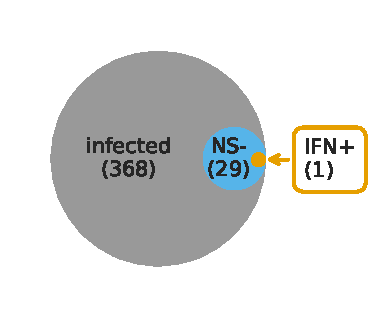
\includegraphics[width=0.25\textwidth,valign=t]{figures/IFN_stochastic/RussellVenn/venn_diagram.pdf}
{\bf \Large B}
{\bf \Large C}
}
\caption{
Triggering of IFN production is rare in influenza-infected cells.
{\bf (A)} Number of influenza-infected, NS-deficient, and IFN+ cells in our prior single-cell study of influenza infection of A549 cells.
The Venn diagram shows data aggregated over all samples from \citet{russell2018extreme}.
{\bf (B)} Number of IFN+ cells in the single-cell analysis of influenza-infected mice by \citep{steuerman2018dissection}.
\jdbcomment{We could possibly add a \emph{small simple} schematic of reporter line here as panel {\bf (C)} and move the current {\bf (C)} to {\bf (D)}, and then have more details in \FIGSUPP[IFNrare]{reporter_cells}.}
Alternatively, we could just show everything in \FIGSUPP[IFNrare]{reporter_cells}.
{\bf (C)} An A549 fluorescent-reporter cell-line confirms that IFN expression is very rare in cells infected with our relatively pure viral stock.
\jdbcomment{This should be a simple figure, such as a plot that just shows the fraction IFN+ among flu infected cells for a few replicates.
If you have suitable data, you could show for low, medium, and high-inducing stock and indicate which we use.
Then put detailed flow data similar to what is in your writeup in \FIGSUPP[IFNrare]{flow}. For that flow data, I think contour plots are better than overplotting. Also, don't subsample but show all points, as that will give better statistics.}
}
\label{fig:IFNrare}

\figsupp[Creation and validation of A549 fluorescent-reporter cell lines for type I and type III IFN expression.]
{CAPTION}
{IMAGE}
\label{figsupp:reporter_cells}

\figsupp[Expression of type I and type III IFN are highly correlated in influenza-infected A549 cells.]
{CAPTION}
{IMAGE}
\label{figsupp:type_I_vs_III}

\figsupp[Full flow cytometry data for \FIG{IFNrare}C.]
{CAPTION}
{IMAGE}
\label{figsupp:flow}

\end{figure}
%%% end IFNrare figure %%%

All past single-cell transcriptomics of viral infected cells~\citep{russell2018extreme,zanini2018single,steuerman2018dissection,zanini2018virus} have focused on counting the number of viral transcripts rather than determining their full sequences.
We came up with a scheme to determine full genotypes of infecting viruses in IFN+ cells (\FIG{approach}).

%%% start approach figure
\begin{figure}

\centerline{\jdbcomment{FIGURE}}

\caption{
{\bf (A)} Schematic of experimental approach.
{\bf (B)} Some summary stats on numbers of cells, etc.
}

\end{figure}
%%% end approach figure


\subsection{Viral genotypes in IFN+ and IFN- influenza-infected cells}
\FIG{genotypes} and \FIGSUPP[genotypes]{genotypes_by_ifn} and \FIGDATA[genotypes]{genotypes}


%%% start genotypes figure %%%
\begin{figure}
\begin{fullwidth}
{\centering
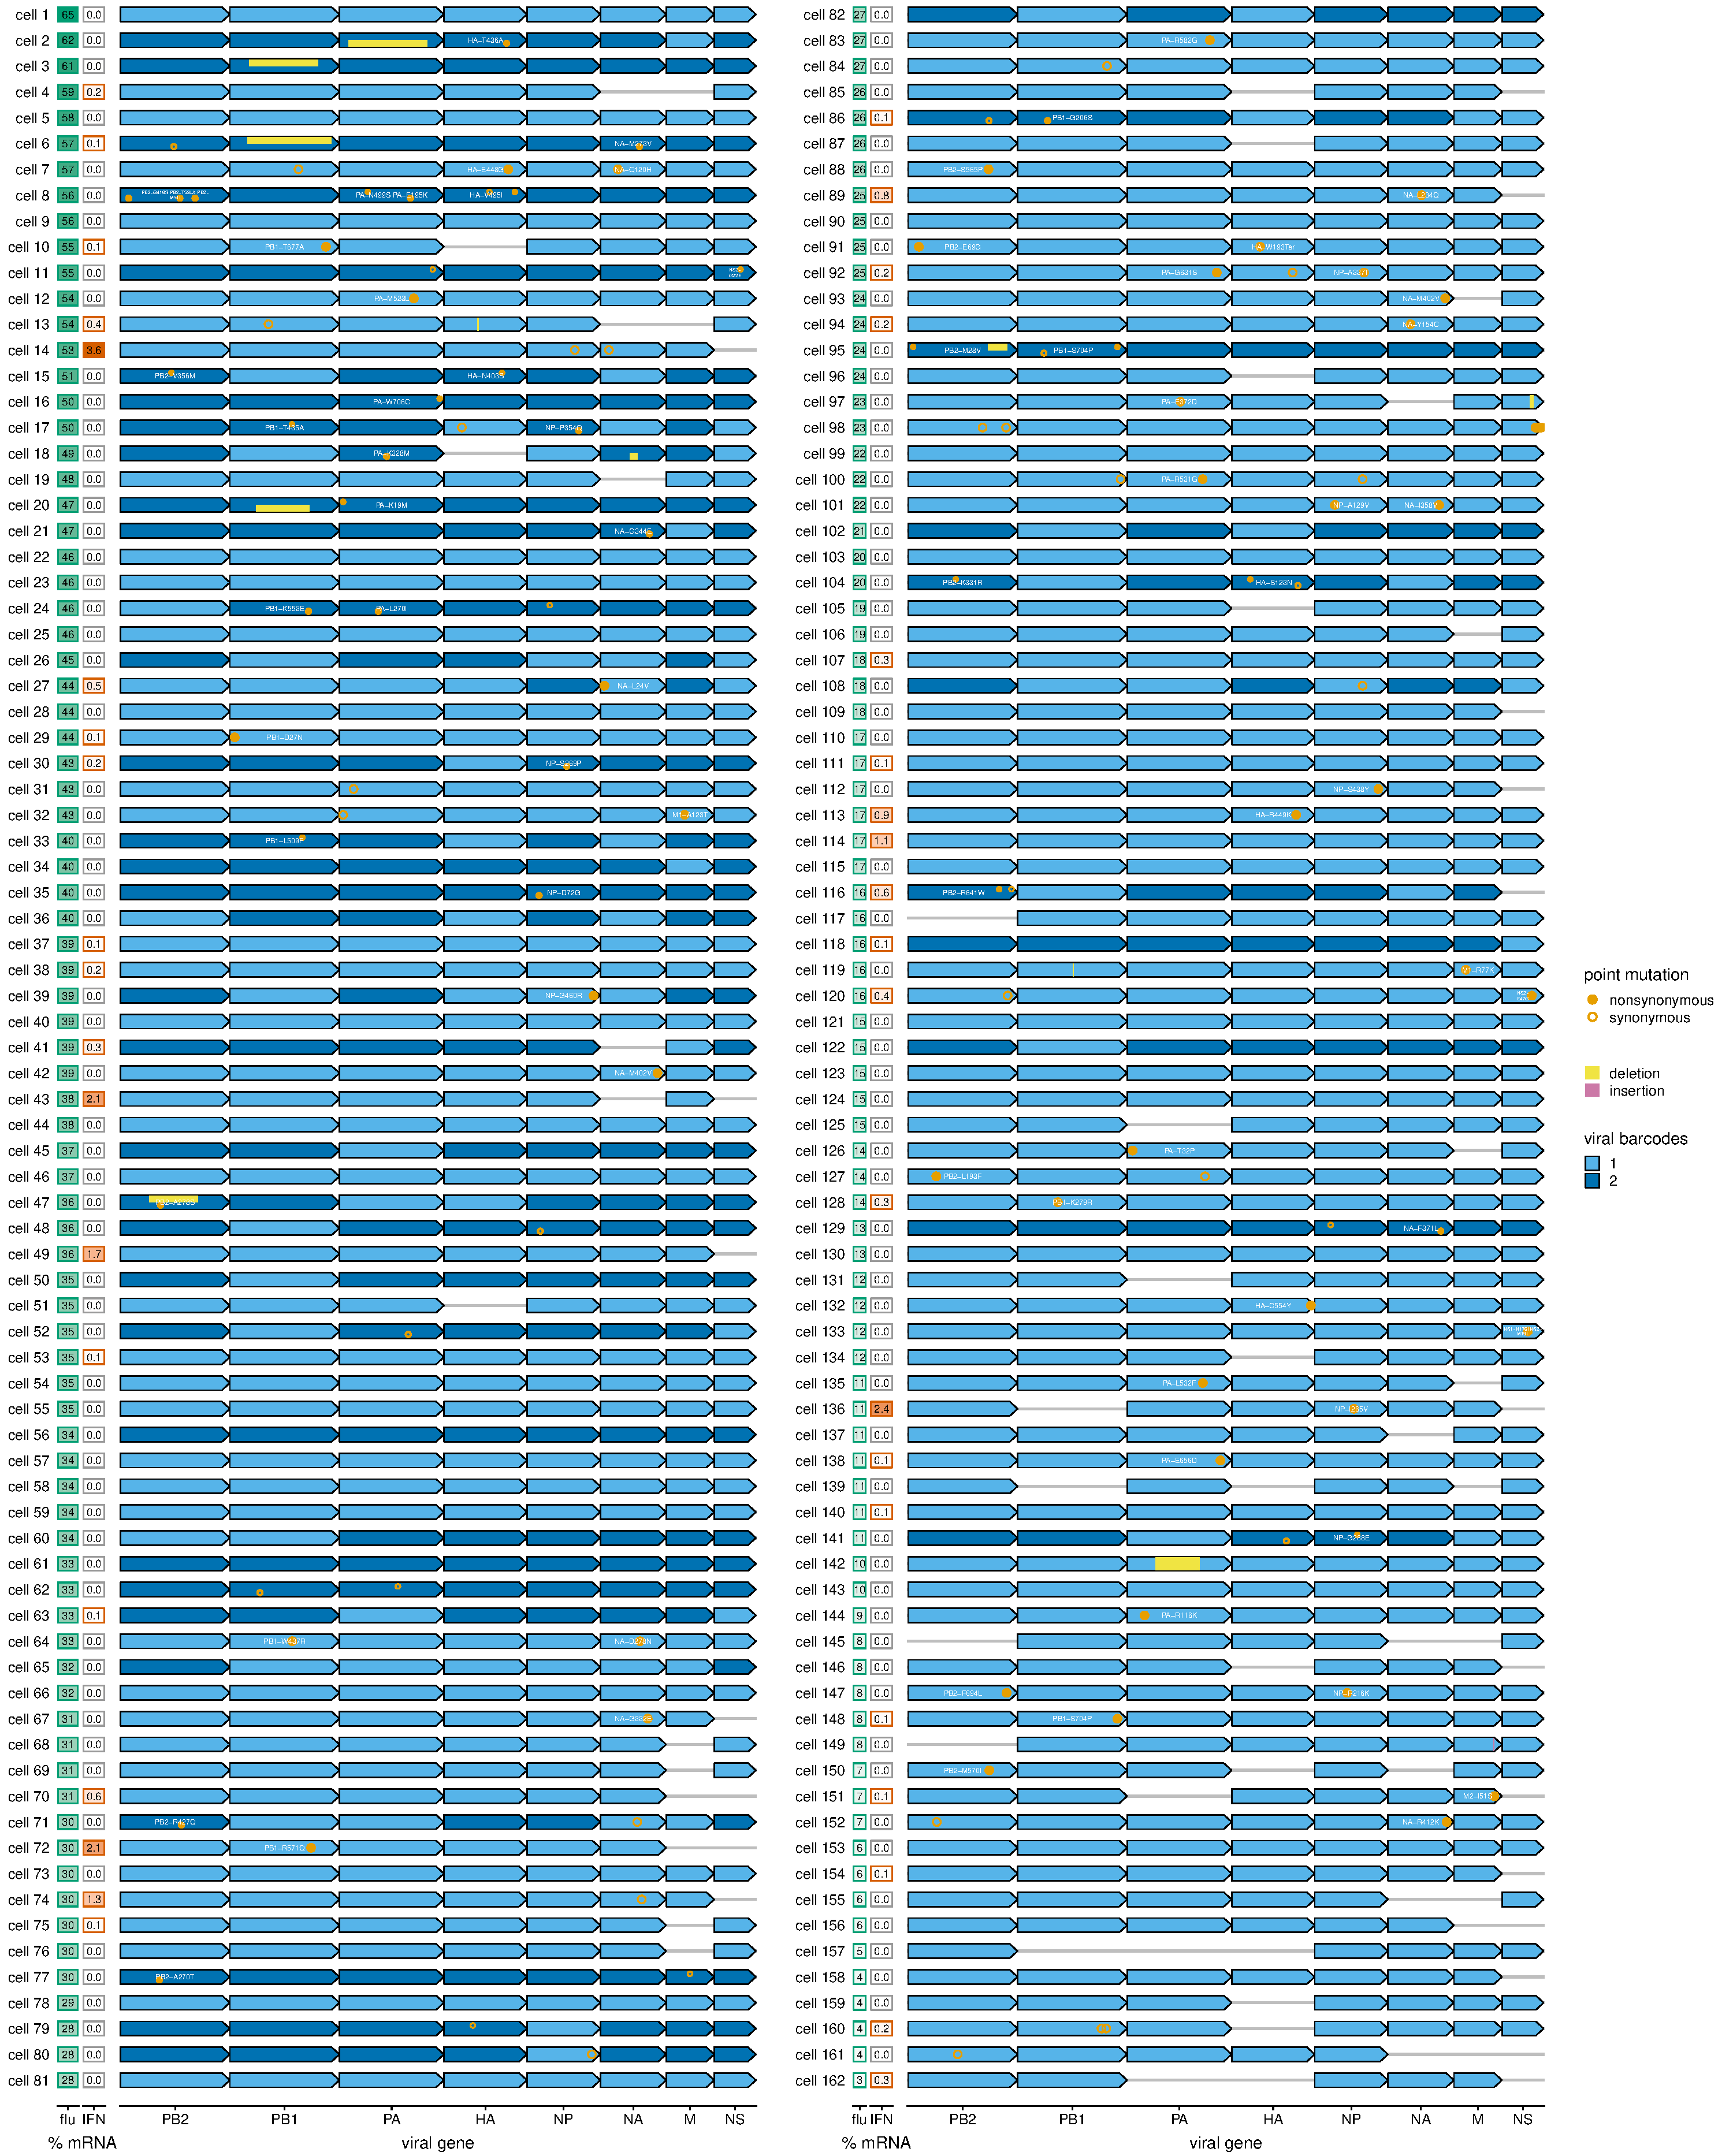
\includegraphics[width=0.9\linewidth]{figures/p_genotypes.pdf}
}
\caption{
Viral genotypes and infection outcomes in single cells.
}
\label{fig:genotypes}

\figsupp[Genotypes and infection outcomes plotted separately for IFN+ and IFN- cells.]
{This plot shows the same data as \FIG{genotypes}, but with cells separated into columns based on whether they are IFN- or IFN+.}
{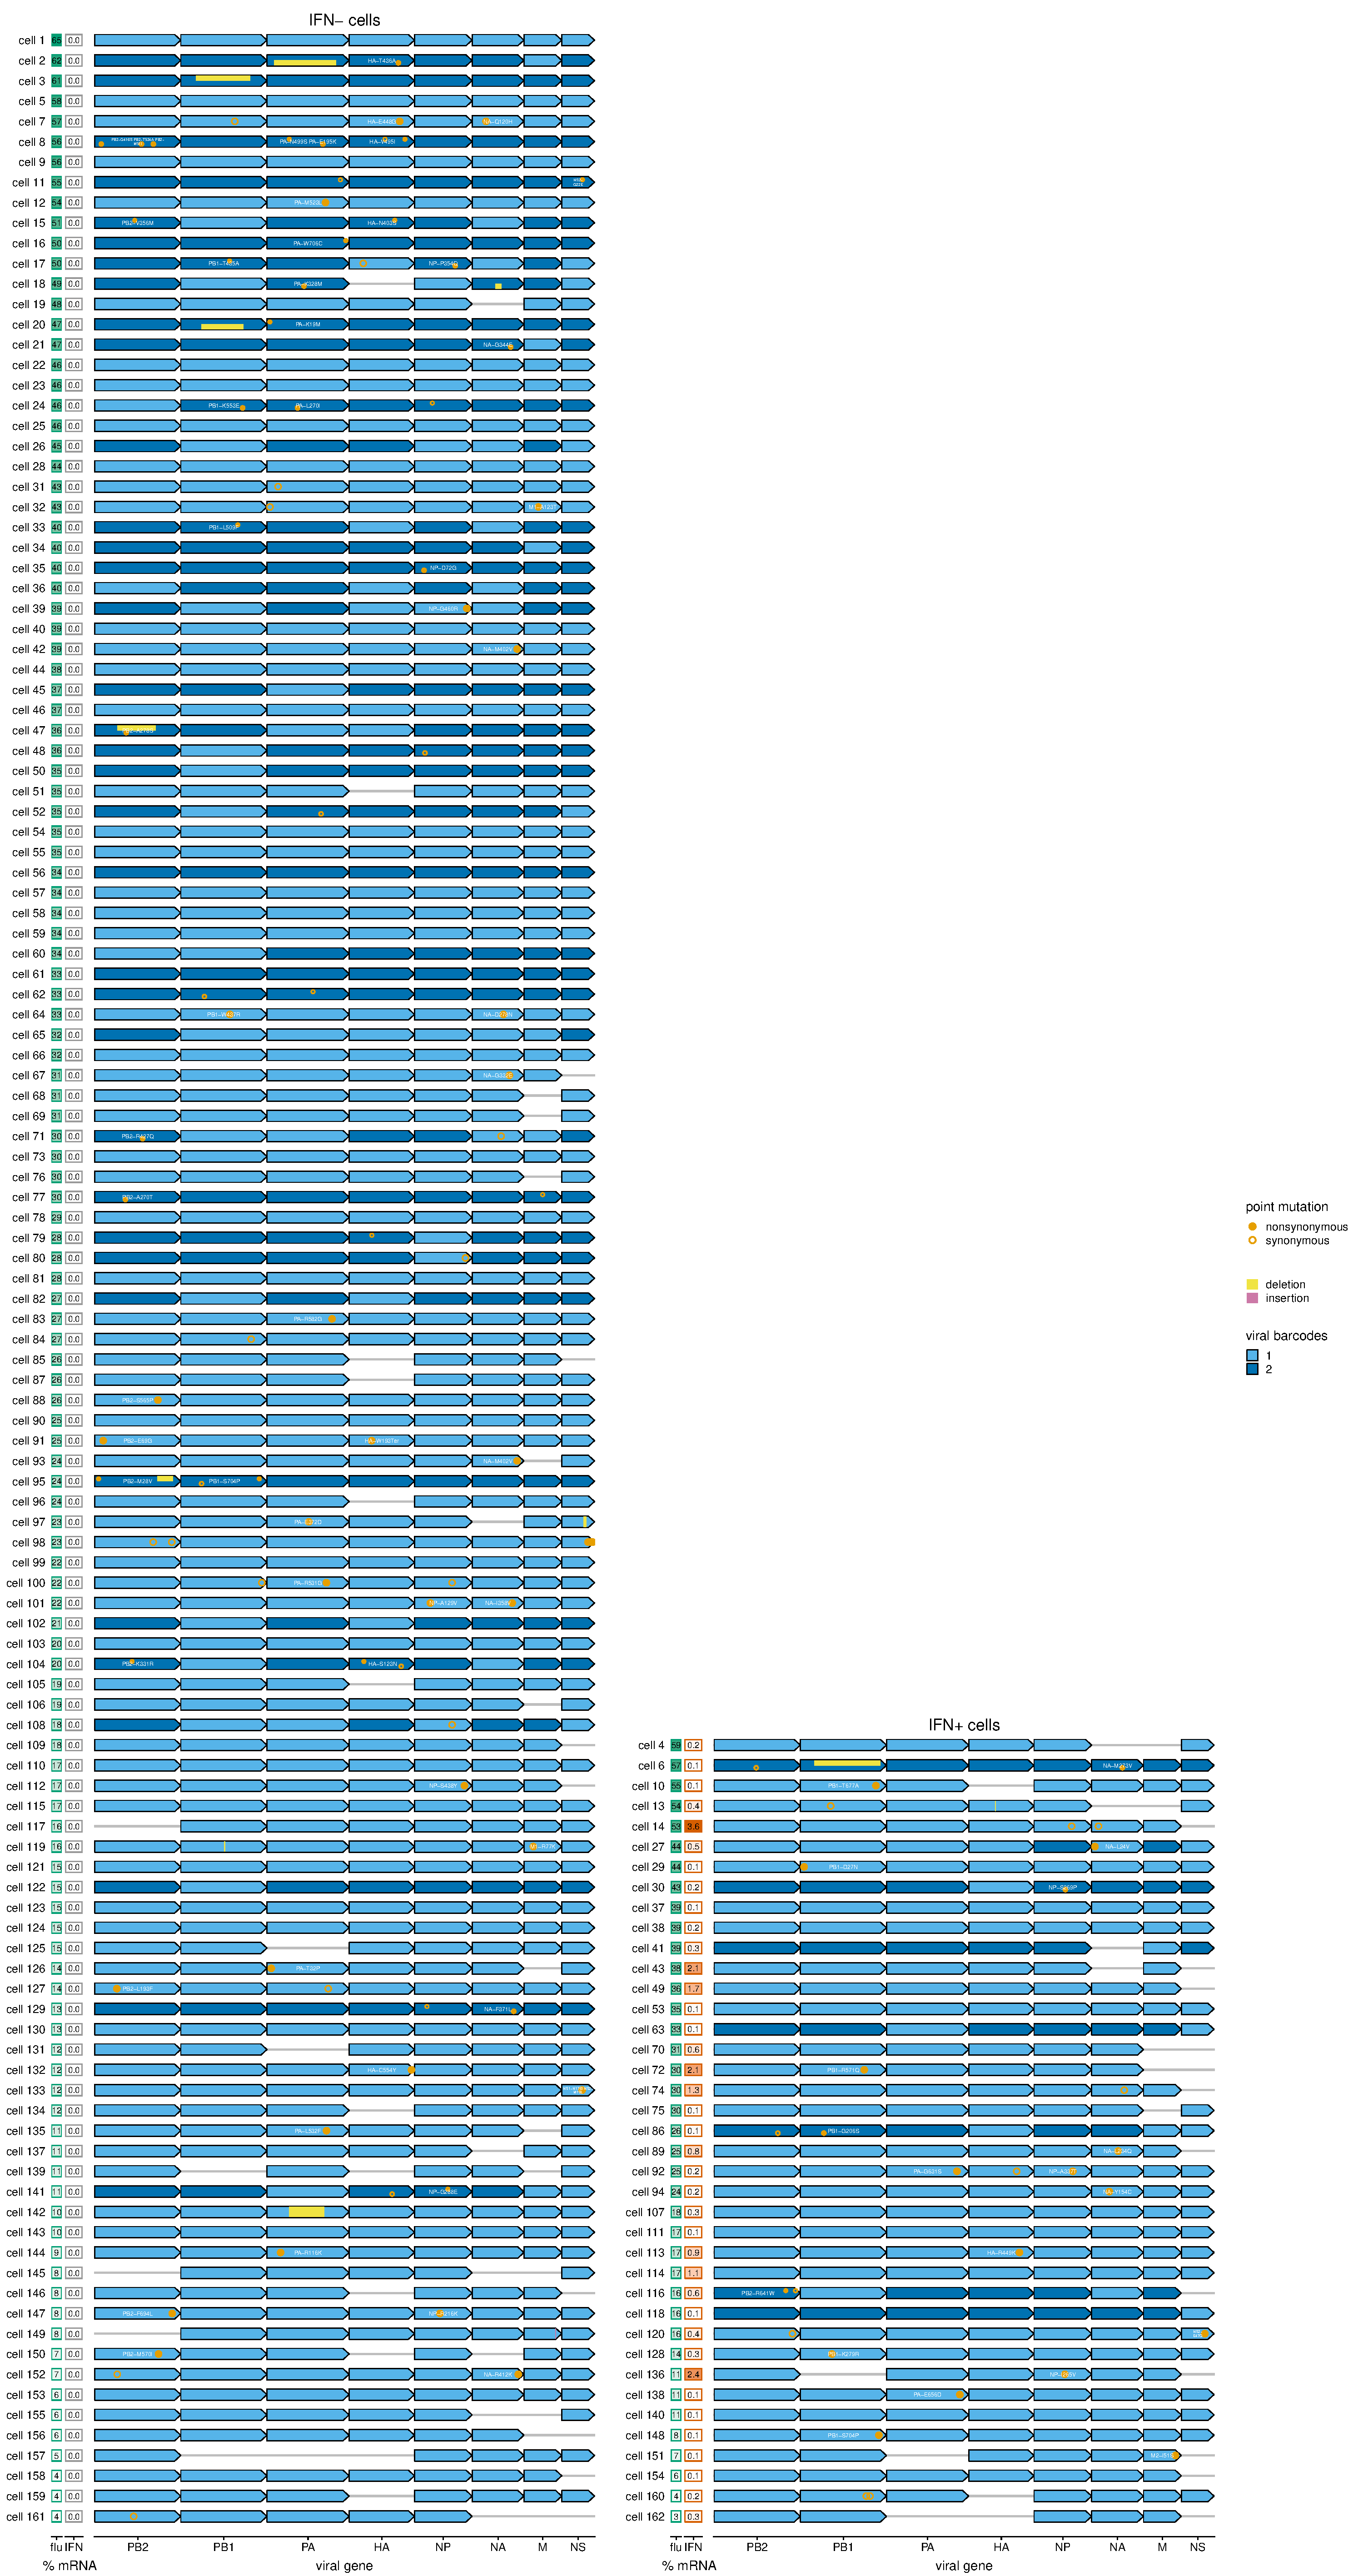
\includegraphics[height=0.95\textheight]{figures/p_genotypes_by_ifn.pdf}}
\label{figsupp:genotypes_by_ifn}

\figdata{A CSV file giving the genotypes is in \texttt{figures/genotypes.csv}.}
\label{figdata:genotypes}

\end{fullwidth}
\end{figure}
%%% end genotypes figure %%%

\section{Discussion}

Add text

\section{Methods and Materials}

Add text




\section{Acknowledgments}

Add this

\nolinenumbers

\bibliography{references}

\end{document}
